% CAPITOLO 2 — STORYBOARDS
\chapter{Storyboards}
\label{cap:storyboards}

\section{Autenticazione e Area Personale}

\subsection{Autenticati}
La schermata di accesso permette all'utente di autenticarsi inserendo le proprie credenziali (email e password).
\begin{figure}[H]
    \centering
    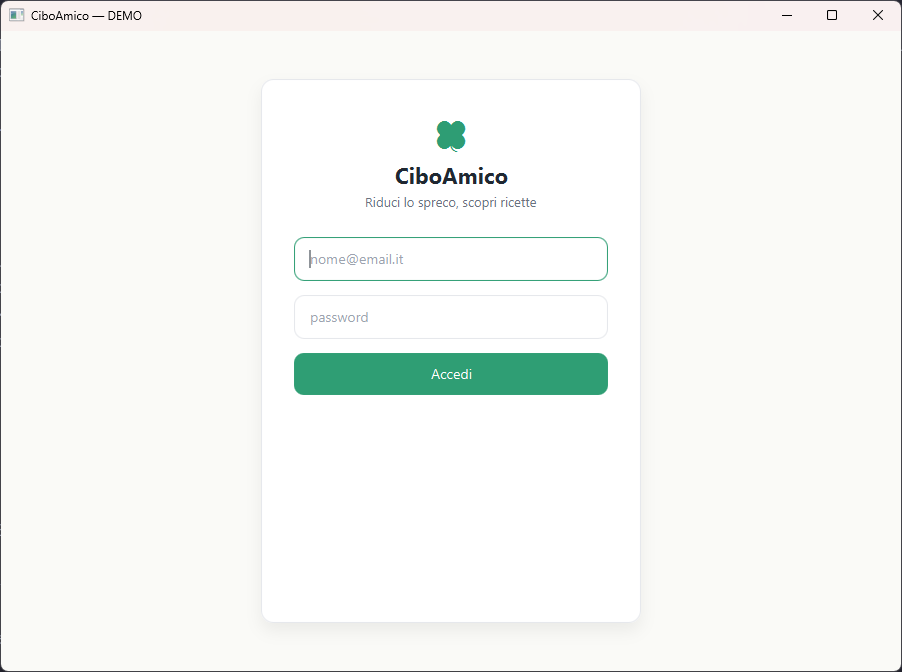
\includegraphics[width=0.8\textwidth]{figures/schermata-login.png}
    \caption{Schermata di autenticazione al sistema.}
    \label{fig:sb_login}
\end{figure}

\subsection{Home (Cliente)}
Completata l'autenticazione, il Cliente raggiunge la dashboard principale (Home). Da qui può raggiungere le funzionalità dell'applicazione: Ricette, Inventario, Lista Spesa e Marketplace (UC-04 Ordina un Prodotto).
\begin{figure}[H]
    \centering
    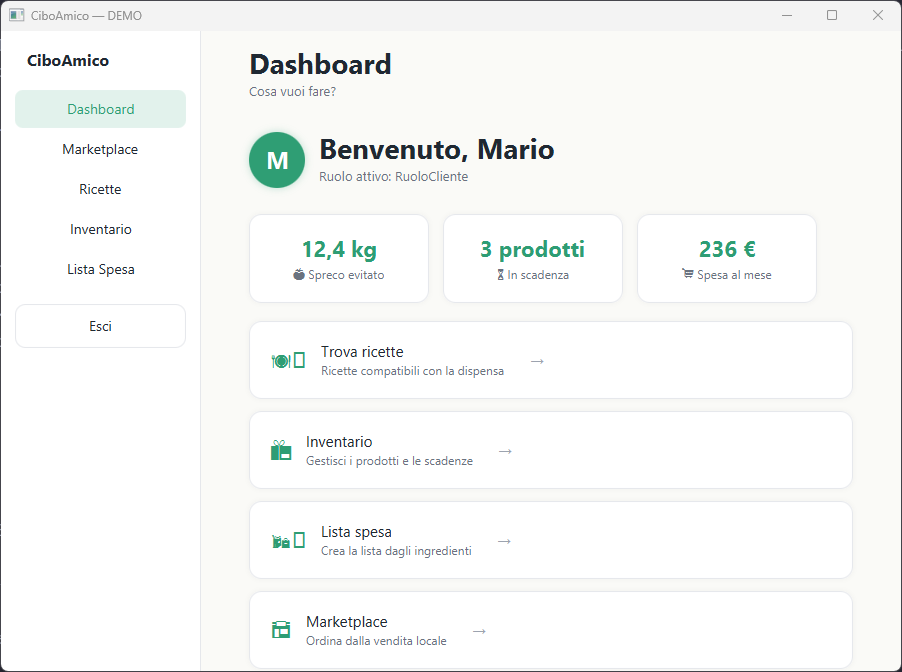
\includegraphics[width=0.8\textwidth]{figures/schermata-home.png}
    \caption{Dashboard principale: accesso alle funzionalità dell'applicazione.}
    \label{fig:sb_home}
\end{figure}

\section{Acquisti e Marketplace (UC-04 Ordina un Prodotto)}

\subsection{Marketplace (Catalogo Prodotti)}
L'area dedicata all'acquisto diretto mostra il catalogo dei prodotti locali dei venditori. Il pannello laterale consente di selezionare un prodotto da ordinare e, opzionalmente, un buono promozionale.
\begin{figure}[H]
    \centering
    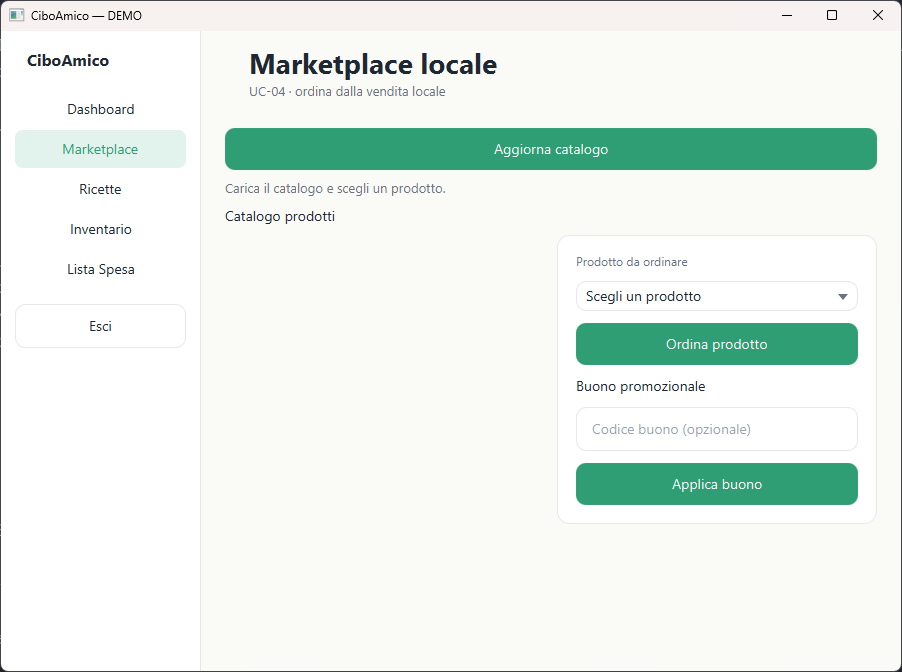
\includegraphics[width=0.8\textwidth]{figures/schermata-marketplace.png}
    \caption{Marketplace: catalogo dei prodotti locali e pannello di acquisto.}
    \label{fig:sb_marketplace}
\end{figure}

\subsection{Ordina un Prodotto}
Selezionato un prodotto dal catalogo e caricata la lista (pulsante \emph{Aggiorna catalogo}), il Cliente sceglie il prodotto nel pannello \emph{Prodotto da ordinare}. Se inserisce un codice buono e preme \emph{Applica buono}, il sistema valida il buono e ricalcola il totale applicando lo sconto (estensione \emph{Ordina un Prodotto}); con \emph{Ordina prodotto} procede.
\begin{figure}[H]
    \centering
    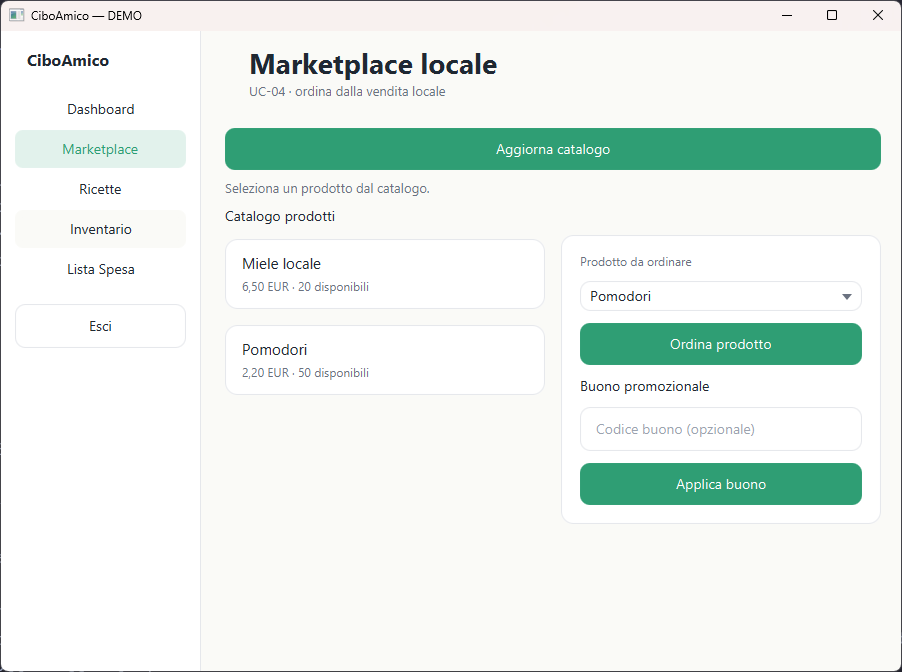
\includegraphics[width=0.8\textwidth]{figures/schermata-ordine.png}
    \caption{Schermata di acquisto con prodotto selezionato e campo buono promozionale.}
    \label{fig:sb_ordine}
\end{figure}

\subsection{Pagamento (passo 6)}
Confermato l'ordine, l'interfaccia passa alla schermata di pagamento: l'utente inserisce i dati della carta (numero, intestatario, scadenza e CVV) e autorizza l'addebito; l'esito è mostrato inline nella stessa vista, come richiesto dall'estensione \textbf{6a} (pagamento rifiutato) del caso d'uso.
\begin{figure}[H]
    \centering
    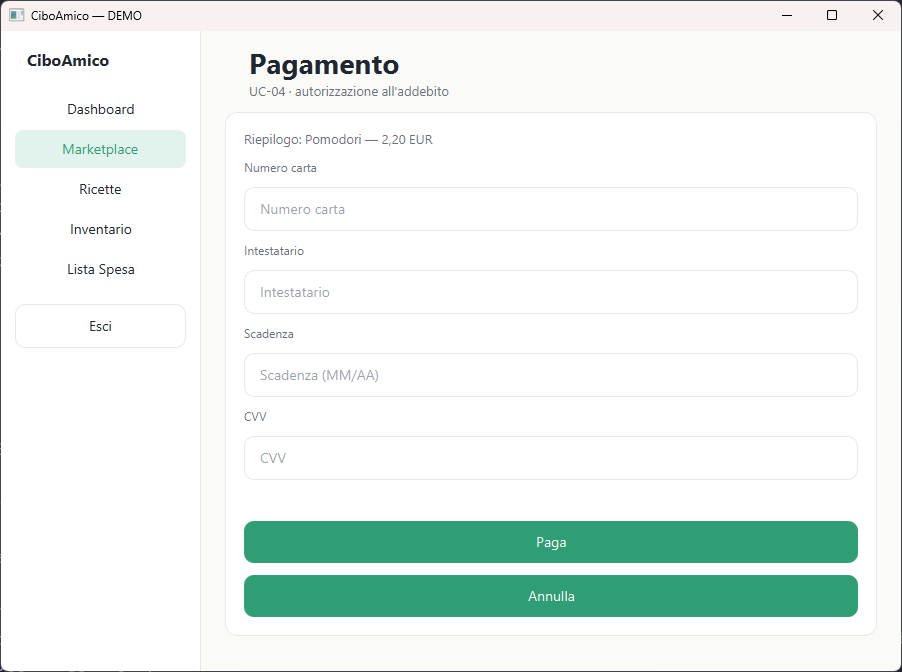
\includegraphics[width=0.8\textwidth]{figures/schermata-payment.png}
    \caption{Schermata di pagamento (dati carta e autorizzazione all'addebito).}
    \label{fig:sb_payment}
\end{figure}
